%%%%%%%%%%%%%%%%%%%%%%%%%%%%%%%%%%%%%%%%%
% Short Sectioned Assignment
% LaTeX Template
% Version 1.0 (5/5/12)
%
% This template has been downloaded from:
% http://www.LaTeXTemplates.com
%
% Original author:
% Frits Wenneker (http://www.howtotex.com)
%
% License:
% CC BY-NC-SA 3.0 (http://creativecommons.org/licenses/by-nc-sa/3.0/)
%
%%%%%%%%%%%%%%%%%%%%%%%%%%%%%%%%%%%%%%%%%

%----------------------------------------------------------------------------------------
%	PACKAGES AND OTHER DOCUMENT CONFIGURATIONS
%----------------------------------------------------------------------------------------

\documentclass[paper=a4, fontsize=11pt]{scrartcl} % A4 paper and 11pt font size

\usepackage[T1]{fontenc} % Use 8-bit encoding that has 256 glyphs
\usepackage{fourier} % Use the Adobe Utopia font for the document - comment this line to return to the LaTeX default
\usepackage[english]{babel} % English language/hyphenation
\usepackage{amsmath,amsfonts,amsthm} % Math packages
\usepackage{hyperref} % For links hyper reference?
\usepackage{lipsum} % Used for inserting dummy 'Lorem ipsum' text into the template
\usepackage{graphicx} % It used for working with graphics. It helps you to include png images into your LaTeX.
\usepackage{minted} % It is used for syntax highlighting, it is bit harder than listings package, you need to have python installed in your system, and you also need to install pygments. If it doesn't work for you try and replace it with listings package.
%\usepackage{listings}
\graphicspath{./Figures} % We are adding the figure's path to our path so that we don't need to write Figure/figure_name.ext in our figure? Does that make sense to you?

\usepackage{sectsty} % Allows customizing section commands

\allsectionsfont{\centering \normalfont\scshape} % Make all sections centered, the default font and small caps
\usepackage{booktabs} % It allows to use books tables. A cool tables
\usepackage{fancyhdr} % Custom headers and footers
\pagestyle{fancyplain} % Makes all pages in the document conform to the custom headers and footers
\fancyhead{} % No page header - if you want one, create it in the same way as the footers below
\fancyfoot[L]{} % Empty left footer
\fancyfoot[C]{} % Empty center footer
\fancyfoot[R]{\thepage} % Page numbering for right footer
\renewcommand{\headrulewidth}{0pt} % Remove header underlines
\renewcommand{\footrulewidth}{0pt} % Remove footer underlines
\setlength{\headheight}{13.6pt} % Customize the height of the header

\numberwithin{equation}{section} % Number equations within sections (i.e. 1.1, 1.2, 2.1, 2.2 instead of 1, 2, 3, 4)
\numberwithin{figure}{section} % Number figures within sections (i.e. 1.1, 1.2, 2.1, 2.2 instead of 1, 2, 3, 4)
\numberwithin{table}{section} % Number tables within sections (i.e. 1.1, 1.2, 2.1, 2.2 instead of 1, 2, 3, 4)

\setlength\parindent{0pt} % Removes all indentation from paragraphs - comment this line for an assignment with lots of text

%----------------------------------------------------------------------------------------
%	TITLE SECTION
%----------------------------------------------------------------------------------------

\newcommand{\horrule}[1]{\rule{\linewidth}{#1}} % Create horizontal rule command with 1 argument of height

\title{	
\normalfont \normalsize 
\textsc{university, school or department name} \\ [25pt] % Your university, school and/or department name(s)
\horrule{0.5pt} \\[0.4cm] % Thin top horizontal rule
\huge Assignment Title \\ % The assignment title
\horrule{2pt} \\[0.5cm] % Thick bottom horizontal rule
}

\author{John Smith} % Your name

\date{\normalsize\today} % Today's date or a custom date

\begin{document}

\maketitle % Print the title

%----------------------------------------------------------------------------------------
%	PROBLEM 1
%----------------------------------------------------------------------------------------

\section{Problem title}

As we have said in the section, your document consists of sections, each section can have many subsection. You can use that by simply typing \emph{\section{The Name of You Section Goes Here}}. For subsections, you need to add the prefix ``sub'' to your section e.g., \emph{\subsection{Some Sub-Section}}. You can go wildly about that, but in practice you only need to use three levels of sections. That is \emph{\subsubsection{Blah Blah Blah}}.\\
That is really what can be said about sections.

\subsection{Ordered and Unordered lists in LaTeX}
The use case of lists is fairly well known. You often need to use ordered lists (with numbers on them), or unordered lists. When you use a command that requires multiple lines you need to use it in the environment `mode'.
For the ordered lists you need to use the \textit{itemize} environment.

\begin{verbatim}
\begin{enumerate}
\item Item 1
\item 2
...
\end{enumerate}
\end{verbatim}

Which produces a list like this one

\begin{enumerate}
	\item Item 1
	\item 2
	...
\end{enumerate}

For the unordered lists, you need to use \textit{itemize} environment.
\begin{verbatim}
\begin{itemize}
\item Item 1
\item 2
...
\end{itemize}
\end{verbatim}

Which then produces this list. As a quick quiz, try to nest these items, that is for each item in your list, make some subitems in it (I might have actually given to you the command for that!). The output should be something like this one.

\begin{itemize}
	\item Item 1
	\subitem Subitem 1
	\subitem Subitem 2
	\item Item 2
	\subitem Subitem 1
	\subitem Subitem 2 
	...
\end{itemize}

\subsection{Equations and Math modes}
There are a few commands in \LaTeX that requires to be in math mode. There are two math modes in \LaTeX
\begin{itemize}
	\item Inline mode e.g., This is $\lambda$, you can access it via the \verb=$\lambda$=, or you can also use \verb=\(\lambda\)=. Both works fine, though I prefer the latter, as it less buggy than the first one (I often tend to forget to include the other dollar sign)
	\item And there is the other other math mode. I do not know exactly what its name, but we can call `the other mode'. The other mode is basically used when you are writing an equation for instance, or any large math expressions. Unlike the inline mode, it actually print your math expression in the middle of your page (and also adds to it the numbering, if you want that)
	\begin{align}
		x &= y^2\\
		z &= x + y
	\end{align}
\end{itemize}

Writing an equation in \LaTeX is fairly easy, you are highly recommended to use amsmath package (which comes with all of your assignments templates). We will only go through the align environment from amsmath package, it is your turn to look through other equations commands available from amsmath package. Suppose that we are trying to solve \(\left(x+y\right)^3\). The split command, though it is not necessary, is used to split your equations into smaller peaces which then will be aligned together. 

\begin{verbatim}
	\begin{align} 
	\begin{split}
	(x+y)^3 	&= (x+y)^2(x+y)\\
	&=(x^2+2xy+y^2)(x+y)\\
	&=(x^3+2x^2y+xy^2) + (x^2y+2xy^2+y^3)\\
	&=x^3+3x^2y+3xy^2+y^3
	\end{split}					
	\end{align}
\end{verbatim}

And it will produce the following nice equations. Notice that we use the ampersand sign \& to \textit{vertically} align our equations at that position. You are generally need to align your equations at the equal sign.

\begin{align} 
\begin{split}
(x+y)^3 	&= (x+y)^2(x+y)\\
&=(x^2+2xy+y^2)(x+y)\\
&=(x^3+2x^2y+xy^2) + (x^2y+2xy^2+y^3)\\
&=x^3+3x^2y+3xy^2+y^3
\end{split}					
\end{align}

That is really all about equations. For very long equations you can use \verb|\multline| environment. We will not discuss it here.

\subsection{Arrays}
Arrays are very important, you often need to use them in Geodesy, or in engineering in general. There are several matrices like parentheses, or brackets, or curly brackets. There are other type, but these are the common ones.
This is an example of a parentheses matrix. 
\begin{verbatim}
\begin{align}
A = \begin{pmatrix}
31 & 4242 & 42 \\
42 & 434 & 4242\\
\end{pmatrix}
\end{align}
\end{verbatim}
You should now get familiar with LaTeX syntax. We want to insert a matrix, so we enter to math environment. Because the matrix are commonly long, they cannot be entered (they can be in fact, but it is not how inline mode is defined), in the inline mode, so we need to enter to the ``other mode". For that, we use the \verb|align| environment. Then, for the parentheses, we use the environment \verb|pmatrix|. If you want to explore other types of matrices, you can replace \verb|pmatrix| with \verb|Bmatrix| (for the curly brackets), or \verb|bmatrix| (for the brackets). There are also other types of matrices are left for you to discover.
\begin{align}
A = \begin{pmatrix}
A_{11} & A_{12} & A_{13}\\
A_{21} & A_{22} & A_{23}
\end{pmatrix}
\end{align}

\subsection{Working with Tables and Figures}
Tables and figures are called floats in LaTeX. They are float because you actually cannot predict where exactly LaTeX will output them. Make sure that you never say at some section ``in the table below''. For that you need to specify a \textit{caption} for your figure, and a \textit{label} so that you can describe exactly what is this figure about, and call it any where from your document. For the tables, we will use the \textit{booktabs} package which gives you nice formatted tables (like those you see in textbooks). Make sure you add it to header of your document (after your documentclass, obviously).

To make a booktabs table, you need to work with two environments. \verb|table| environment allows you to work with general properties of a table e.g., its position, the caption and, its label. In the label, the convention is to first write the name of the float e.g., table, followed by colon, and then the id of it. Try to give it some meanigful name, something that you can remember later (my-table-2) is really a bad one.\\
After that, we use the tabular environment from booktabs to give us the textbooks tables style. The tabular environment needs to know the number of your \textit{columns} beforehand, in out case we use l's as indicator for the number of our columns. That is two l's mean that our table will have two columns. The @{} are used for styling purposes only. They add extra spaces for your table, so that it looks better, you can use them, or you can totally ignore them. The table consists of three horizontal lines (from now on, I will call them horizontal rules). There are three commands for them because each one of them has a different styling. They are \verb|\toprule|, \verb|midrule|, and \verb|\bottomrule|, respectively. As you can see from Table \ref{table:my-table-2}, there are two rules that seperates the header from the table contents. Review this code to better understand how the table is generated.

\begin{verbatim}
\begin{table}
\centering
\caption{This is a very nice table}
\label{table:my-table-2}
\begin{tabular}{@{}lll@{}}
\toprule
\emph{Column1} & \emph{Column2} & \emph{Column1}\\
\midrule
some-data & another one & again\\
42 & 43 & 43\\
42 & 42 & 42\\
\bottomrule
\end{tabular}
\end{table}
\end{verbatim}

\begin{table}
	\centering
	\caption{This is a very nice table}
	\label{table:my-table-2}
	\begin{tabular}{@{}lll@{}}
		\toprule
		\emph{Column1} & \emph{Column2} & \emph{Column1}\\
		\midrule
		some-data & another one & again\\
		42 & 43 & 43\\
		42 & 42 & 42\\
		\bottomrule
	\end{tabular}
\end{table}

I've noticed that I'm horrible at generating random numbers.\\
Because it is very hard to enter all the tables numbers, I've developed a tool to convert NumPy arrays into LaTeX tables, you can download it using \mint{shell}{pip install array2latex}. There are other tools like \href{http://www.tablesgenerator.com/}{Tables Generator}. But you need to use VPN to access it, that why I've built array2latex tool.\\

\paragraph{Quiz} Your quiz for this part is to find how to write vertical tables in LaTeX, those are generally used when you have too many columns. (I'm not sure though whether they are called vertical tables or not)
\\
Using figures is also pretty straight forward. Again, we need to specify the caption, the label and the position of the figure. You can also resize your figure, so that it will not take too much place from your figure. We have already added the `Figure' directory to your path so that you do not need to add it when you specify the figure name using \verb|\includegraphics{imagefile}| command.

\begin{verbatim}
	\begin{figure}
	\centering
	\caption{In this figure we are demonstrating something.}
	\label{Figures/figure:my-figure} % Remember that we have added the figure path to our current directoy. For me it didn't work so I had to use the full path.
	\includegraphics{classic_style.png }
	\end{figure}
\end{verbatim}

\begin{figure}
	\centering
	\caption{In this figure we are demonstrating something.}
	\label{figure:my-figure}
	\includegraphics{Figures/classic_style.png}
\end{figure}

That is all about figures in LaTeX.

%------------------------------------------------

\subsection{Using Syntax Highlighting}

Minted is a very cool package to highlight your code. It is installation might be a little bit harder (in Linux environment, at least). First you need to have a Python installed on your system and also a python's package called pygments. If you do not have Python installed, please go to Anaconda website and download a version from them (you can download it from the official website, however Anaconda gives you a whole punch of Python's scientific packages pre-built for you--which is something very hard to do in Windows). Having done that, open your shell (or command line), and type on it \mint{shell}{pip install pygments}. You need to have an internet connection as it needs to download the files. If everything goes right, you are good to go!


\begin{minted}{python}
	def somefunction(a, b, c):
	    """This is a very cool function, is not it?"""
	    return a * b* c
\end{minted}

It is very cool and it has so many nice features and a rich set of themes (you can search for pygments and see their themes). To create the previous code snippest you need to use \verb|minted| environment, and pass to it the language that your code is about to highlight it the right way.

\begin{verbatim}
\begin{minted}{python} % This is a python code, however you use MATLAB to highlight MATLAB's ones, if you want that.
def somefunction(a, b, c):
"""This is a very cool function, is not it?"""
return a * b* c
\end{minted}
\end{verbatim}

\begin{align}
A = 
\begin{bmatrix}
A_{11} & A_{21} \\
A_{21} & A_{22}
\end{bmatrix}
\end{align}

\section{Collaboration}
As we have said in the section, you are highly encouraged to work together, but you have to make sure that \textit{all} of your submission is yours! We have very strict collaboration policy, so please make sure that you anything your submit is yours, and whenever you used someone's work you clearly indicate that (by citing them).\\
Another important thing, whenever you have collaborated with someone, please write down their names. Having done will save you from getting zero marks. There is no penalty of writing the names of people you have worked with them--they won't also get any credit for that--it's just for us to know that you have worked together. Again, working together does \textit{not} mean giving someone's your code!\\
Another thing, we need to know the hours you have spent on working with each assignment, so that we can know exactly if it is too much (or too little!). Please provide correct answers, I mean we will give you any extra credits if you solve your assignment in one hour! It is just for us to make sure that we are not giving you too much.
\\

\textbf{I've collaborated with:} ................\\
\textbf{Approximate hours for this assignment}:......... hours
\\

Last thing, the previous part of the collaboration and hours should always be on the bottom of your assignment.\\


 

\end{document}